\begin{document}

\begin{flushleft}
    {\Huge \textbf{Discrete Dislocation Dynamics}} \\[0.2cm]
    {\Huge \textbf{simulation}}
\end{flushleft}

% Changed \section to \chapter or \section* depending on book class behavior. 
% Using \section* to behave more like the original PDF structure while in 'book' class.
\section*{1 Introduction}
\addcontentsline{toc}{section}{1 Introduction}

Many models have been developed to understand and predict the plastic behaviour of crystals. Similar to mechanism behind plasticity, these models also vary widely in length and time scales as depicted in Figure \ref{fig:scales}. In previous practicals we introduced the Molecular Dynamics (MD) and Continuum Mechanics (CM) as simulation tools for nano and macro scales. In the length scales from 100s nm to 10s $\mu$m the size of the specimen is comparable with the size of dislocations and therefore the dislocations dominate the mechanical response of material. In this length scale MD simulations are numerically infeasible and continuum mechanics does not have enough information to accurately predicts the behaviour of crystals. We close the gap between these two scales by introducing Discrete Dislocations Dynamic simulation (DDD). The main ingredient of DDD simulations are dislocations.


\begin{figure}[htbp]
  \centering
    
% Define the specific blue colors from the image
\definecolor{boxblue}{RGB}{91, 136, 198}
\definecolor{boxborder}{RGB}{68, 103, 149}

\begin{tikzpicture}[
    box/.style={
        draw=boxborder,
        thick,
        fill=boxblue,
        rounded corners=3.5mm,
        text=white,
        font=\Large\bfseries,
        align=center,
        inner sep=0pt
    }
]
% Axes
\draw[->, ultra thick] (0.5, 1) -- (11, 1);
\draw[->, ultra thick] (1, 0.5) -- (1, 7.8);

% Axis titles
\node at (6, -0.2) {\large\textbf{length}};
\node[rotate=90] at (-0.2, 4.4) {\large\textbf{time}};

% Y-axis labels
\node at (0.5, 2.1) {\Large\textbf{ps}};
\node at (0.5, 3.3) {\Large\textbf{ns}};
\node at (0.5, 4.6) {\Large\textbf{$\mu$s}};
\node at (0.5, 6.2) {\Large\textbf{s}};

% X-axis labels
\node at (1.4, 0.5) {\Large\textbf{\AA}};
\node at (4.0, 0.5) {\Large\textbf{nm}};
\node at (6.8, 0.5) {\Large\textbf{$\mu$m}};
\node at (9.4, 0.5) {\Large\textbf{m}};

% Stacking the boxes from bottom-left to top-right
\node[box, minimum width=2.6cm, minimum height=1.8cm] at (2.6, 2.1) {QM};
\node[box, minimum width=2.8cm, minimum height=1.9cm] at (4.5, 3.3) {MD};
\node[box, minimum width=3.0cm, minimum height=2.1cm] at (6.5, 4.6) {Mesoscale\\[0.5ex](DDD)};
\node[box, minimum width=3.4cm, minimum height=2.4cm] at (8.7, 6.2) {Microscale\\[0.5ex](CM)};

\end{tikzpicture}

  \caption{Time and size scales for differnt simulation methods \cite{cazacu_discrete_2008}}
  \label{fig:scales}
\end{figure}

Dislocations are one of the most important defects in the crystalline materials. A dislocation is a line defect which caused by the permanent deviations of atoms from their original crystallographic periodicity. Under the applied stresses a dislocation line segment can move, rotate and expand. The motion of dislocations due to the applied stresses produces the plastic deformation in crystals. In other word, dislocations are the boundaries of the plastically slipped regions in the crystal.

The collective motion and interaction of dislocations defines the mechanical behaviour of the crystals. Therefore modelling the plastic behaviour of crystalline materials involves resolving the dislocations interactions at the atomistic scale and also evaluating the deformations at the macroscopic scale.

\section*{2 Discrete Dislocation dynamics Simulation}
\addcontentsline{toc}{section}{2 Discrete Dislocation dynamics Simulation}

The Discrete dislocation dynamics (DDD) are the simulation tools for predicting the movement and interaction of dislocations. In a DDD simulation, dislocations are represented by line segments in a 3-dimensional volume. These dislocations are border of plastic slips in the crystal and therefore induce a stress field around them. The Dislocation segments interact through these stress fields. All DDD frameworks share a common underlying algorithm:
\begin{enumerate}
    \item evaluating the stress field (which consists of external stresses and dislocations stresses) in the simulation domain.
    \item evaluating the acting forces on the dislocation line segments.
    \item moving the dislocation segments according to theses forces.
\end{enumerate}

In this Practicals we use microMegas discrete dislocation dynamic package. microMegas (also known as 'mM') is an open source program for Dislocation Dynamics simulations to model the plastic behaviour of crystalline materials using the elastic theory of dislocations \cite{devincre2011}.

A dislocation is not necessarily a straight line in the simulation cell. Due to the interaction with the other dislocations it can bow out and become a curved line. Different methods have been incorporated to represent the curved dislocation segments. In microMegas a curved segment is discretized into several straight segments. The start and the end nodes of these segments are located on the discrete dislocation lattice. A dislocation segment is defined by the coordinates of its origin, a vectorial length and velocity.

microMegas (mM) uses eight different types of dislocation segments containing pure edge and screw dislocations as well as mixed dislocations (Figure \ref{fig:vectors}).

\begin{figure}[htbp]
  \centering
      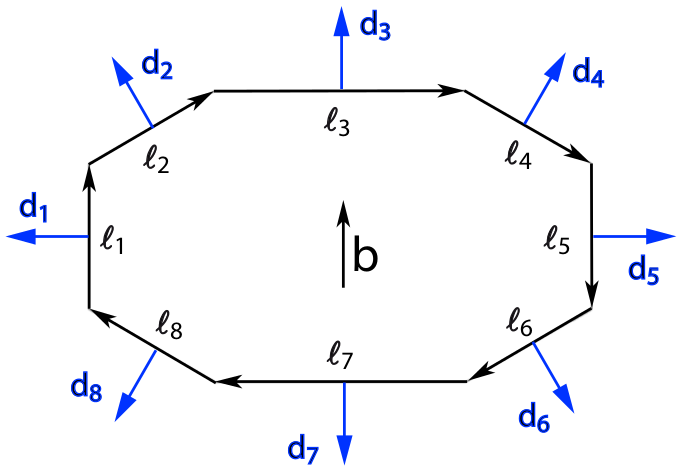
\includegraphics[width=0.9\linewidth]{extracted_image-004.png}
  \caption{Schematic representation of the elementary vectors used per slip system to discretize dislocation lines in mM. The vectors $l_i$ (in black), are used for the definition of the segments directions and the vectors $d_i$ (in blue) for the corresponding displacement directions\cite{devincre2011}}
  \label{fig:vectors}
\end{figure}

The Peach-Köhler equation
\begin{equation}
F = (\sigma_{ext} + \sigma_{int}) b l
\end{equation}
calculates the force F on a dislocation line arising from external $\sigma_{ext}$ and internal stresses $\sigma_{int}$, with Burgers vector b and the line vector l. This equation must be solved repeatedly for all dislocation segments at all time steps. External stresses are prescribed on the simulation cell. Internal stresses arise from the long range interactions between dislocations and can not be neglected at any distance. Having the forces acting on the dislocation segments one can calculate the velocities by
\begin{equation}
v = M(F)
\end{equation}

using a mobility function $M(F)$. The mobility function depends on the orientation of the dislocation segment and the material and takes resistive forces like the Peierls barrier or phonon drag into account. The position of the segments after a time increment $\Delta t$ can then be calculated by time integration. Assuming quasi-static deformation conditions the dislocations move with steady-state velocity and the explicit forward Euler can be used to calculate the new position
\begin{equation}
r(t+\Delta t) = r(t) + v(t)\Delta t
\end{equation}
As dislocation lines evolve their length may change or they might become curved lines. In order to have an exact representation of the dislocation lines in the next time step new nodes must be added or close nodes get merged and removed accordingly.

\section*{3 Frank-Read Source}
\addcontentsline{toc}{section}{3 Frank-Read Source}

One of the main mechanism of dislocation generation in the bulk of FCC crystals is Frank-Read source. A Frank-Read source is a dislocation segment whose ends are pinned by precipitates or because the dislocation leaves the glide plane (Figure \ref{fig:fr_source}).

Under strong enough resolved shear stress the segment bows out by glide motion. The force acting on the initial dislocation segment (a) is given by Peach-Koehler equation
\begin{equation}
F = \tau \cdot bl
\end{equation}
where b is the burgers vector and l is the distance between pinned ends of the dislocation. This force F acts perpendicularly to the dislocation line segment, inducing the dislocation to lengthen and curve into an arc (b). The bending force caused by the shear stress is opposed by the line tension of the dislocation, which acts on each end of the dislocation along the direction of the dislocation line away from A and B with a magnitude of $\mu b^2$, where $\mu$ is the shear modulus. 

Below a critical stress the line tension forces balances with applied stress and dislocation will stay in a metastable equilibrium configuration(c). As an increasing external force is applied the segment bows out until it reaches an unstable semicircle configuration where the line tension is maximum. Once the semicircle configuration is reached no additional increase in external force is needed to further extend the segment(d). Below a critical stress the line tension force balances the applied stress and dislocation will stay in a metastable equilibrium configuration. For the large bow-out case this equilibrium

\begin{figure}[htbp]
  \centering
      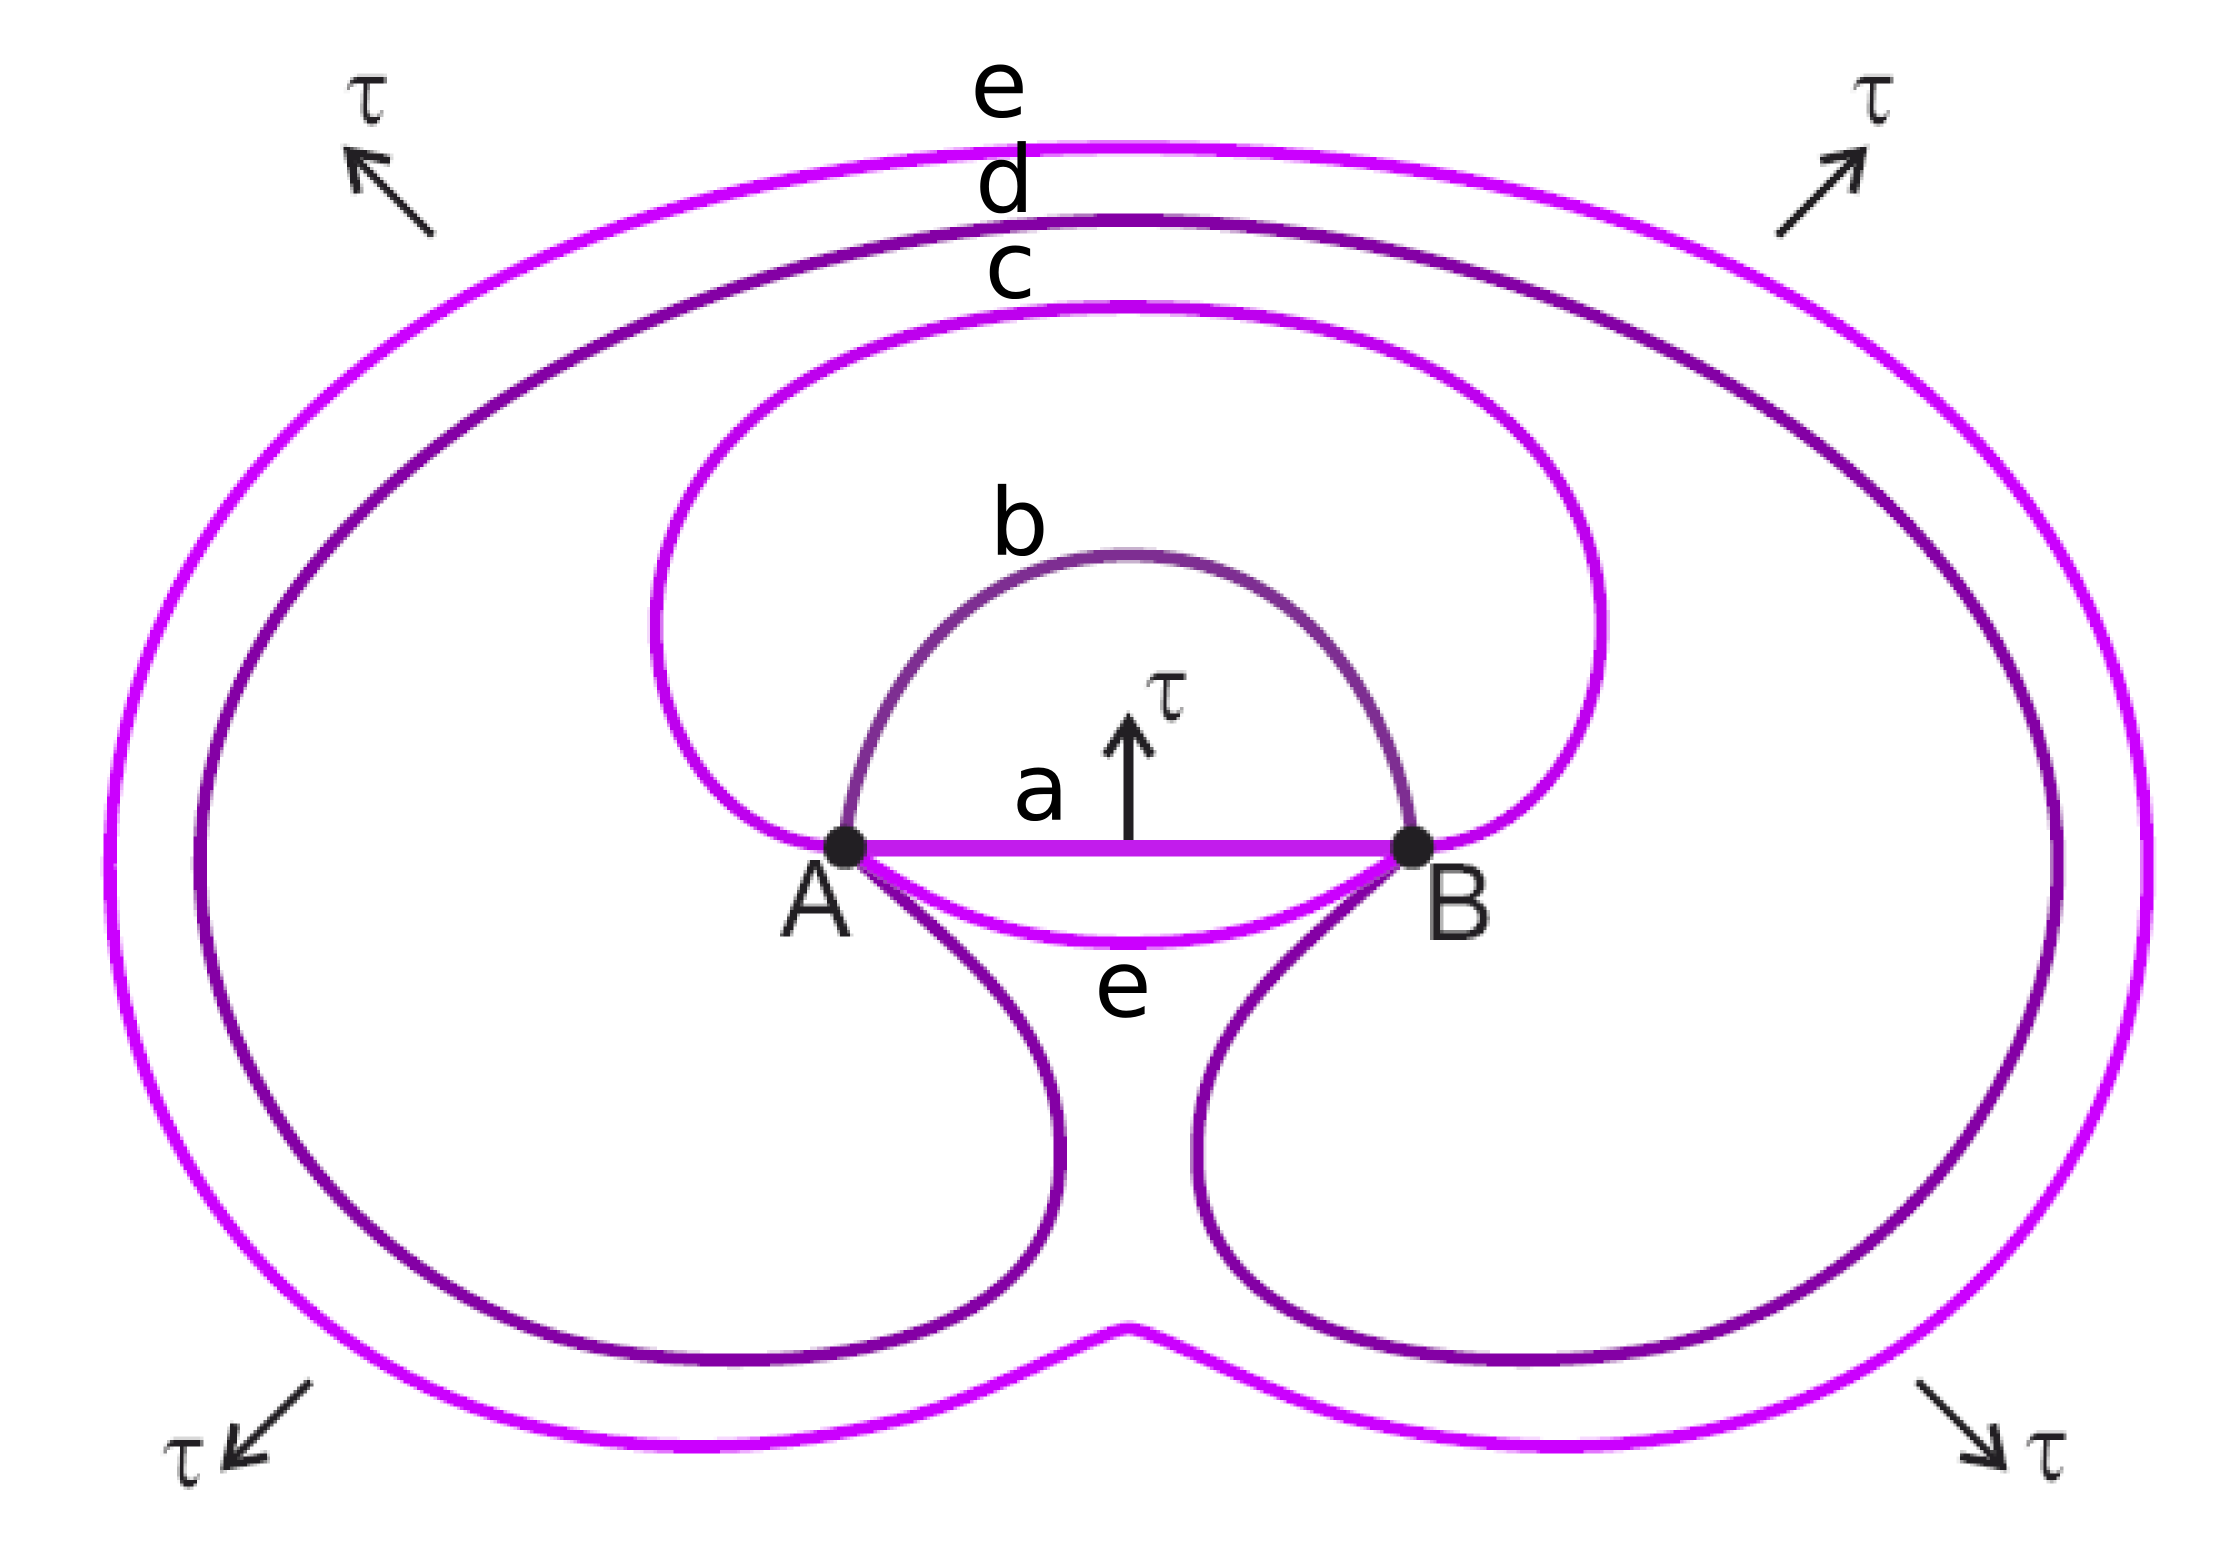
\includegraphics[width=0.4\linewidth]{extracted_image-008.png}
  \caption{Activation of a Frank-Read source: Dislocation segment (a) is pinned at point A and B. Under the applied shear stress $\tau$ it starts to bow out (b) till it reaches its critical configuration (c), and then expands through its unstable state (d) till self-anihilates to a dislocation loop and a new FR segment (e).}
  \label{fig:fr_source}
\end{figure}

stress is given by Hirth (\cite{anderson2017}, P. 752):
\begin{equation}
b\tau_{crit} = \frac{\mathcal{T}}{r} = \frac{\mu b^2}{4\pi r(1-\nu)} \left\{ \left[ 1 - \frac{\nu}{2}(3 - 4\cos^2\beta) \right] \ln\frac{L}{\rho} - 1 + \frac{\nu}{2} \right\}
\end{equation}
where r is the radius of the loop and $\beta$ is the angel between original dislocation line direction and the burgers vector. The radius of the curvature is a minimum when $r = L/2$. Hence the maximum stress for which local equilibrium is possible is given by the equation above with $r = L/2$. For the typical case that $L = 1000\rho$ and $\mu = 0.33$, the critical stress for a dislocation initially pure edge and pure screw, respectively, is $\tau_{crit} = 0.5\mu b/L$ and $\tau_{crit} = 1.5\mu b/L$. Equation 5 can be simplified to:

\begin{equation}
\tau_{crit} = \alpha \frac{\mu b}{L}
\label{eq:tau_crit}
\end{equation}
where $\alpha$ is a geometrical factor depending on the initial line segment orientation and the material properties. As bowing out continues, the two side of the dislocation arms with opposite dislocation vector converge. Finally these arms annihilate, a dislocation loop forms and the original pinned dislocation segment is restored (e). Thus Frank Read sources are able to emit an infinite number of dislocation loops until internal stresses or relaxation of elastic stresses drop the shear stress below the critical point (Figure \ref{fig:surface_fr}).

\begin{figure}[htpb]
  \centering
      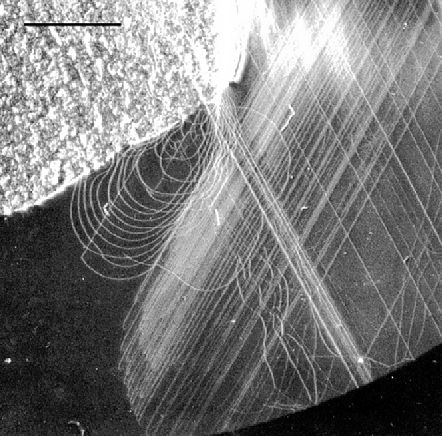
\includegraphics[width=0.3\linewidth]{extracted_image-011.png}
  \caption{A surface frank-Read source in Si crystal is activated many time.}
  \label{fig:surface_fr}
\end{figure}

\newpage
\section*{4 Tasks}
\addcontentsline{toc}{section}{4 Tasks}

In this practicals we use microMegas to conduct some parameter studies on Frank-Read sources. The first step is to get familiar with mM framework and setting up the problem.

\begin{tcolorbox}[colback=white,colframe=black,sharp corners,boxrule=0.5pt]
\textbf{\hypertarget{task1}{Task 1: Setup the simulation of the Frank-Read source in mM:}}
\label{task:one}
\begin{enumerate}
    \item Clone the Repository for the mM from Github \url{https://github.com/LAPikachu/practical_DDD}.
    \item Read the README instructions.
    \item To run a standard DD simulation, one traditionally needs to manually define three input files in the \texttt{input.dd} file: the material variables file (e.g. \texttt{Cu}), the control parameters file (e.g. \texttt{ContCu}), and the initial dislocation configuration file (e.g. \texttt{SegCu}). Instead of manual configuration, check the \texttt{SimulationConfig} dataclass in the Python wrapper and find out which parameters can be set in it to generate these files automatically.
    \item Set up a single FCC crystal using Copper material properties. Use the wrapper to set the simulation box size to $3 \mu m \times 3 \mu m \times 3 \mu m$.
    \item Define a pinned edge dislocation segment with 100 nm length in the $\hkl(-1-1-1)$ slip plane with a Burgers vector of   $\hkl[10-1]$.
    \item Estimate the critical activation stress.
    \item Run the simulation via the Python wrapper with a range of applied stresses close to your estimation and find the critical shear stress.
    \item Determine the parameter $\alpha$ in equation \ref{eq:tau_crit}.
\end{enumerate}

\begin{lstlisting}[language=Python, caption=Minimal microMegas Python Wrapper Implementation]
from micromegas_wrapper import MicroMegasWrapper, SimulationConfig

# Initialize the wrapper pointing to the local repository
wrapper = MicroMegasWrapper(base_repo_path="./practical_DDD")

# Define the minimum required simulation parameters
run_config = SimulationConfig(
    target_seg_length_nm=100.0,
    angle_deg=90,           # Angle between dislocation and burgers vector
    box_dim_x=3000,         # Target dimensions in nanometers
    box_dim_y=3000,         
    box_dim_z=3000,         
    sigma0_mpa=53.6,        # Applied initial stress (MPa)
    use_graphics=False      # Set to True to trigger the graphical interface
)

# Execute the simulation and retrieve the CSV output path
csv_output_path = wrapper.run(run_config)

print(f"Simulation complete. Data exported to: {csv_output_path}")
\end{lstlisting}

\end{tcolorbox}

After setting up mM we are ready to start the parameter study. Equation \ref{eq:tau_crit} shows that the critical shear stress is inversely proportional to the initial dislocation segment length. We investigate this property in the next task.

\begin{tcolorbox}[colback=white,colframe=black,sharp corners,boxrule=0.5pt]
\textbf{Task 2: Investigate the dependency of critical shear stress on the initial dislocation segment length.}
\begin{enumerate}
    \item Start from the simulation setup of the \hyperlink{task1}{Task 1}
    \item Change the length if the initial dislocation line segment gradually from 50nm to 200nm.
    \item For each length find the critical shear stress by running the simulation around expected values.
    \item Plot the simulation results and analytical solution together with the relative error.
    \item Find out for which line length the simulation matches the analytical solution better. Explain your findings.
    \item Investigate which simulation parameters (simulation box size, minimum segment length, ...) are affecting the simulation results.
\end{enumerate}
\end{tcolorbox}

The parameter $\alpha$ depends on the initial dislocation line orientation w.r.t burgers vector. In the next task we investigate this correlation.

\begin{tcolorbox}[colback=white,colframe=black,sharp corners,boxrule=0.5pt]
\textbf{Task 3: Investigate the dependency of critical shear stress on the initial segment line orientation.}
\begin{enumerate}
    \item Start from the simulation setup of the \hyperlink{task1}{Task 1}
    \item Change the initial dislocation line orientation gradually from (+edge -$>$ +screw). this can be done by changing $\beta$ the angle between dislocation line segment and the burgers vector while dislocation remains on the slip plane. Note that dislocation segments are consisted of only pure edge, screw or mixed segments. You might need to write a small script to generate the correct segments.
    \item For each orientation find the critical shear stress and determine the parameter $\alpha$
    \item plot the parameter $\alpha$ against $\beta$
\end{enumerate}
\end{tcolorbox}

\printbibliography[title={References}]

\end{document}